\documentclass{article}\usepackage[]{graphicx}\usepackage[]{xcolor}
% maxwidth is the original width if it is less than linewidth
% otherwise use linewidth (to make sure the graphics do not exceed the margin)
\makeatletter
\def\maxwidth{ %
  \ifdim\Gin@nat@width>\linewidth
    \linewidth
  \else
    \Gin@nat@width
  \fi
}
\makeatother

\definecolor{fgcolor}{rgb}{0.345, 0.345, 0.345}
\newcommand{\hlnum}[1]{\textcolor[rgb]{0.686,0.059,0.569}{#1}}%
\newcommand{\hlsng}[1]{\textcolor[rgb]{0.192,0.494,0.8}{#1}}%
\newcommand{\hlcom}[1]{\textcolor[rgb]{0.678,0.584,0.686}{\textit{#1}}}%
\newcommand{\hlopt}[1]{\textcolor[rgb]{0,0,0}{#1}}%
\newcommand{\hldef}[1]{\textcolor[rgb]{0.345,0.345,0.345}{#1}}%
\newcommand{\hlkwa}[1]{\textcolor[rgb]{0.161,0.373,0.58}{\textbf{#1}}}%
\newcommand{\hlkwb}[1]{\textcolor[rgb]{0.69,0.353,0.396}{#1}}%
\newcommand{\hlkwc}[1]{\textcolor[rgb]{0.333,0.667,0.333}{#1}}%
\newcommand{\hlkwd}[1]{\textcolor[rgb]{0.737,0.353,0.396}{\textbf{#1}}}%
\let\hlipl\hlkwb

\usepackage{framed}
\makeatletter
\newenvironment{kframe}{%
 \def\at@end@of@kframe{}%
 \ifinner\ifhmode%
  \def\at@end@of@kframe{\end{minipage}}%
  \begin{minipage}{\columnwidth}%
 \fi\fi%
 \def\FrameCommand##1{\hskip\@totalleftmargin \hskip-\fboxsep
 \colorbox{shadecolor}{##1}\hskip-\fboxsep
     % There is no \\@totalrightmargin, so:
     \hskip-\linewidth \hskip-\@totalleftmargin \hskip\columnwidth}%
 \MakeFramed {\advance\hsize-\width
   \@totalleftmargin\z@ \linewidth\hsize
   \@setminipage}}%
 {\par\unskip\endMakeFramed%
 \at@end@of@kframe}
\makeatother

\definecolor{shadecolor}{rgb}{.97, .97, .97}
\definecolor{messagecolor}{rgb}{0, 0, 0}
\definecolor{warningcolor}{rgb}{1, 0, 1}
\definecolor{errorcolor}{rgb}{1, 0, 0}
\newenvironment{knitrout}{}{} % an empty environment to be redefined in TeX

\usepackage{alltt}
\usepackage{amsmath} %This allows me to use the align functionality.
                     %If you find yourself trying to replicate
                     %something you found online, ensure you're
                     %loading the necessary packages!
\usepackage{amsfonts}%Math font
\usepackage{graphicx}%For including graphics
\usepackage{hyperref}%For Hyperlinks
\usepackage[shortlabels]{enumitem}% For enumerated lists with labels specified
                                  % We had to run tlmgr_install("enumitem") in R
\hypersetup{colorlinks = true,citecolor=black} %set citations to have black (not green) color
\usepackage{natbib}        %For the bibliography
\setlength{\bibsep}{0pt plus 0.3ex}
\bibliographystyle{apalike}%For the bibliography
\usepackage[margin=0.50in]{geometry}
\usepackage{float}
\usepackage{multicol}

%fix for figures
\usepackage{caption}
\newenvironment{Figure}
  {\par\medskip\noindent\minipage{\linewidth}}
  {\endminipage\par\medskip}
\IfFileExists{upquote.sty}{\usepackage{upquote}}{}
\begin{document}

\vspace{-1in}
\title{Lab 02 -- MATH 240 -- Computational Statistics}

\author{
  Andrew Li \\
  Affiliation  \\
  Department of Mathematics  \\
  {\tt ali@colgate.edu}
}

\date{}

\maketitle

\begin{multicols}{2}
\begin{abstract}
This experiment seek to analyze how big of an influence did different music groups have on songs, specifically how much did the bands Manchester Orchestra, The Front Bottoms, and All Get Out affect the song ``Allentown." By using Essentia \citep{bogdanov2013essentia}, an open-source program for music analysis and synthesis, the musical components of 180 songs were isolated to be compared with the parts of \texttt{Allentown}. This method would be give more depth into the analysis and provide a better understanding of what elements are extracted from music. Through this process, the steps of data cleaning and summarization will be explored.  

\end{abstract}

\noindent \textbf{Keywords:} Cleaning data, extracting and automating data processing 

\section{Introduction}

Music plays such an important role in everyday lives, from creating social spaces, providing an outlet, and connecting people throughout the world. As a result, the works of different artists can be traced to find influence from older generations or their peers. The song ``Allentown" by Front Bottoms and Manchester Orchestra has influence from the two bands and All Get Out, so this lab seeks to explore what elements are similar and who overall has contributed the most to the creation of this song. There are many ways to conduct this comparison, but musical components was an objective way to analyze in pieces how similar the songs are. To do this, Essentia \citep{bogdanov2013essentia} is going to be used to collect data via music analysis. Since Essentia allows processing on individual tracks, it became neccesary to prepare a batch of json files using the tracks from all the artists. 



\section{Methods}
To replicate this experiment, it is important to make sure to download the jsonlite and stringr \texttt{R} packages. The music directory contained all 181 of the song tracks from the three bands, and we created a program that extracted all the provided .wav files (musical files) and processed them to create the batch file of executable command lines for the Essentia program to run. Using the \texttt{stringr} \citep{st} package for R , we were able to extract information from each wave file and organize each line by artist and album. Following that, we used the \texttt{jsonlite} \citep{js} package to create a sample program that can pull information from the json files that Essentia would return. This preliminary step showed how the larger scale data extraction will work. \\
\indent To get a full picture on which band plays the most influence, we took the data from the Essentia processed calls, drew additional features such as mood from Essentia models \citep{alonso2020tensorflow}, and analyzed thoughts and personality traits through a text analysis tool called LIWC. This was all compiled into one \texttt{csv} file to sort and organize all of our data before we initiated a feature-by-feature comparison to see what insights we can draw about the rise of the song ``Allentown." \\
\indent Using boxplots, a sample analysis was shown for the emotional element and tone for ``Allentown" compared to the tracks from the three bands. 

Using the tidyverse package for \texttt{R} \citep{tidyverse}, it became easier to summerize and visualize our data because of the extensive functionality built into the package. 



\section{Results}
Currently, it is hard to determine what band had a greater influence on the song ``Allentown." By collecting analyzed musical elements and processed components, it becomes possible to see what parts of the song are similar to the works of \textit{Manchester Orchestra}, \textit{All Get Out}, or \textit{The Front Bottoms}. The final product from the data collection and cleaning is presented inside the trainingdata.csv file while the musical components for ``Allentown" is separated inside the testingdata.csv to avoid conflicting overlap.
\newpage



\begin{figure}[H]
\begin{center}
\begin{knitrout}
\definecolor{shadecolor}{rgb}{0.969, 0.969, 0.969}\color{fgcolor}
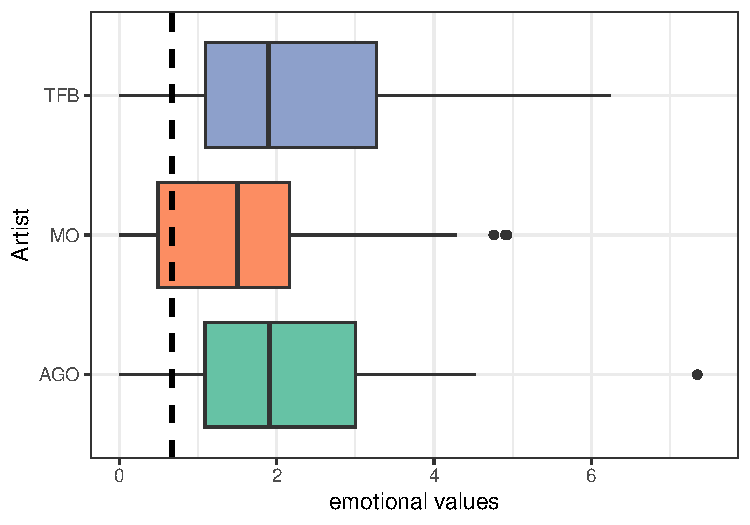
\includegraphics[width=\maxwidth]{figure/unnamed-chunk-1-1} 
\end{knitrout}
\caption{Emotional sound analysis \\ (names are shortened to MO, AGO, and TFB)}
\label{plot1} 
\end{center}
\end{figure}



\section{Discussion}
  Given the sample analysis, a fair guess would be that The Front Bottoms has a bigger influence based on Figure 1 since the IQR is higher up; however, if the guess is based on figure 2, then Manchester Orchestra would have more influence since its range is the lowest of the three bands and the emotion value for ``Allentown" sits right inside the IQR for Manchester Orchestra. However, more analysis would be needed to infer any direct correlation. 




%%%%%%%%%%%%%%%%%%%%%%%%%%%%%%%%%%%%%%%%%%%%%%%%%%%%%%%%%%%%%%%%%%%%%%%%%%%%%%%%
% Bibliography
%%%%%%%%%%%%%%%%%%%%%%%%%%%%%%%%%%%%%%%%%%%%%%%%%%%%%%%%%%%%%%%%%%%%%%%%%%%%%%%%
\vspace{2em}


\begin{tiny}
\bibliography{bib}
\end{tiny}
\end{multicols}

\begin{table}[H]
\centering
\begin{tabular}{rlrrrrlll}
  \hline
 & artist & minimum & LF & RF & maximum & out.of.range & unusual & description \\ 
  \hline
1 & All Get Out & -14.27 & -16.35 & -5.10 & -6.13 & FALSE & FALSE & Within Range \\ 
  2 & Manchester Orchestra & -24.34 & -20.22 & -5.66 & -6.26 & FALSE & FALSE & Within Range \\ 
  3 & The Front Bottoms & -11.03 & -9.65 & -6.81 & -5.71 & FALSE & TRUE & Unusual \\ 
  4 & All Get Out & 0.02 & 0.01 & 0.04 & 0.05 & FALSE & FALSE & Within Range \\ 
  5 & Manchester Orchestra & 0.01 & -0.00 & 0.04 & 0.05 & FALSE & FALSE & Within Range \\ 
  6 & The Front Bottoms & 0.02 & 0.02 & 0.05 & 0.05 & FALSE & FALSE & Within Range \\ 
  7 & All Get Out & 0.84 & 0.77 & 1.18 & 1.30 & FALSE & FALSE & Within Range \\ 
  8 & Manchester Orchestra & 0.78 & 0.65 & 1.21 & 1.40 & FALSE & FALSE & Within Range \\ 
  9 & The Front Bottoms & 0.91 & 0.86 & 1.24 & 1.33 & TRUE & FALSE & Out of Range \\ 
  10 & All Get Out & 84.91 & 95.29 & 149.76 & 162.92 & FALSE & FALSE & Within Range \\ 
  11 & Manchester Orchestra & 67.15 & 71.18 & 160.30 & 184.57 & FALSE & FALSE & Within Range \\ 
  12 & The Front Bottoms & 80.83 & 82.99 & 157.05 & 165.67 & FALSE & FALSE & Within Range \\ 
  13 & All Get Out & 163.50 & 134.57 & 261.03 & 377.87 & FALSE & FALSE & Within Range \\ 
  14 & Manchester Orchestra & 102.43 & 79.15 & 320.67 & 434.36 & FALSE & FALSE & Within Range \\ 
  15 & The Front Bottoms & 108.49 & 127.14 & 258.48 & 297.35 & FALSE & FALSE & Within Range \\ 
  16 & All Get Out & 0.04 & 0.02 & 0.08 & 0.08 & FALSE & FALSE & Within Range \\ 
  17 & Manchester Orchestra & 0.02 & 0.00 & 0.07 & 0.09 & FALSE & FALSE & Within Range \\ 
  18 & The Front Bottoms & 0.04 & 0.04 & 0.07 & 0.11 & TRUE & TRUE & Out of Range \\ 
  19 & All Get Out & 0.43 & 0.26 & 1.05 & 1.29 & FALSE & FALSE & Within Range \\ 
  20 & Manchester Orchestra & 0.42 & 0.11 & 1.07 & 1.35 & FALSE & FALSE & Within Range \\ 
  21 & The Front Bottoms & 0.52 & 0.38 & 0.99 & 1.36 & FALSE & FALSE & Within Range \\ 
  22 & All Get Out & 2620015.25 & 3162397.09 & 4788882.53 & 4758639.50 & TRUE & TRUE & Out of Range \\ 
  23 & Manchester Orchestra & 1937052.25 & 1668651.00 & 4817223.00 & 5845988.50 & FALSE & TRUE & Unusual \\ 
  24 & The Front Bottoms & 3510343.75 & 3538674.50 & 5508843.50 & 5888673.00 & FALSE & FALSE & Within Range \\ 
  25 & All Get Out & 1.14 & 0.81 & 2.01 & 4.12 & FALSE & TRUE & Unusual \\ 
  26 & Manchester Orchestra & 1.16 & -0.49 & 3.70 & 6.75 & FALSE & FALSE & Within Range \\ 
  27 & The Front Bottoms & 0.87 & 0.63 & 1.96 & 2.04 & TRUE & TRUE & Out of Range \\ 
  28 & All Get Out & 935.91 & 701.91 & 2250.95 & 2520.04 & TRUE & TRUE & Out of Range \\ 
  29 & Manchester Orchestra & 518.87 & 151.27 & 1600.19 & 2566.67 & FALSE & FALSE & Within Range \\ 
  30 & The Front Bottoms & 927.04 & 740.58 & 2001.24 & 3190.29 & TRUE & TRUE & Out of Range \\ 
  31 & All Get Out & 0.00 & 0.00 & 0.01 & 0.01 & FALSE & FALSE & Within Range \\ 
  32 & Manchester Orchestra & 0.00 & 0.00 & 0.01 & 0.01 & FALSE & FALSE & Within Range \\ 
  33 & The Front Bottoms & 0.00 & 0.00 & 0.01 & 0.01 & FALSE & FALSE & Within Range \\ 
  34 & All Get Out & 3.03 & -0.36 & 8.83 & 40.10 & FALSE & TRUE & Unusual \\ 
  35 & Manchester Orchestra & 3.36 & -13.58 & 26.13 & 98.58 & FALSE & TRUE & Unusual \\ 
  36 & The Front Bottoms & 1.89 & 0.00 & 7.16 & 10.47 & TRUE & TRUE & Out of Range \\ 
  37 & All Get Out & 0.04 & 0.05 & 0.10 & 0.10 & FALSE & FALSE & Within Range \\ 
  38 & Manchester Orchestra & 0.02 & 0.01 & 0.10 & 0.11 & FALSE & FALSE & Within Range \\ 
  39 & The Front Bottoms & 0.07 & 0.06 & 0.11 & 0.12 & FALSE & FALSE & Within Range \\ 
  40 & All Get Out & 6.44 & 7.00 & 7.91 & 7.91 & FALSE & TRUE & Unusual \\ 
  41 & Manchester Orchestra & 5.79 & 5.22 & 7.98 & 7.89 & FALSE & FALSE & Within Range \\ 
  42 & The Front Bottoms & 7.11 & 7.10 & 7.85 & 8.02 & TRUE & TRUE & Out of Range \\ 
  43 & All Get Out & 0.01 & 0.00 & 0.01 & 0.02 & FALSE & TRUE & Unusual \\ 
  44 & Manchester Orchestra & 0.00 & 0.00 & 0.02 & 0.02 & FALSE & FALSE & Within Range \\ 
  45 & The Front Bottoms & 0.01 & 0.00 & 0.02 & 0.02 & FALSE & FALSE & Within Range \\ 

   \hline
\end{tabular}
\end{table}

%%%%%%%%%%%%%%%%%%%%%%%%%%%%%%%%%%%%%%%%%%%%%%%%%%%%%%%%%%%%%%%%%%%%%%%%%%%%%%%%
% Appendix
%%%%%%%%%%%%%%%%%%%%%%%%%%%%%%%%%%%%%%%%%%%%%%%%%%%%%%%%%%%%%%%%%%%%%%%%%%%%%%%%


\end{document}
